\section{Methodology}

This section will describe the tools and the methods we used to realise the project.

\subsection{GitHub}

In order to simplify the work as a team we used a GitHub repository. GitHub is a version control repository, in other words it allows people to manage their project files in a simpler way. We decided to work with GitHub because we knew that, during the project, our team would be scattered and it would be difficult to meet in order to work together. Indeed GitHub makes the current version of the project available for all the members of the team simultaneously. As you can see in the following figure GitHub makes it easy to see what everyone has done so far and what might be left to do (or not working).


\begin{figure}[H]
	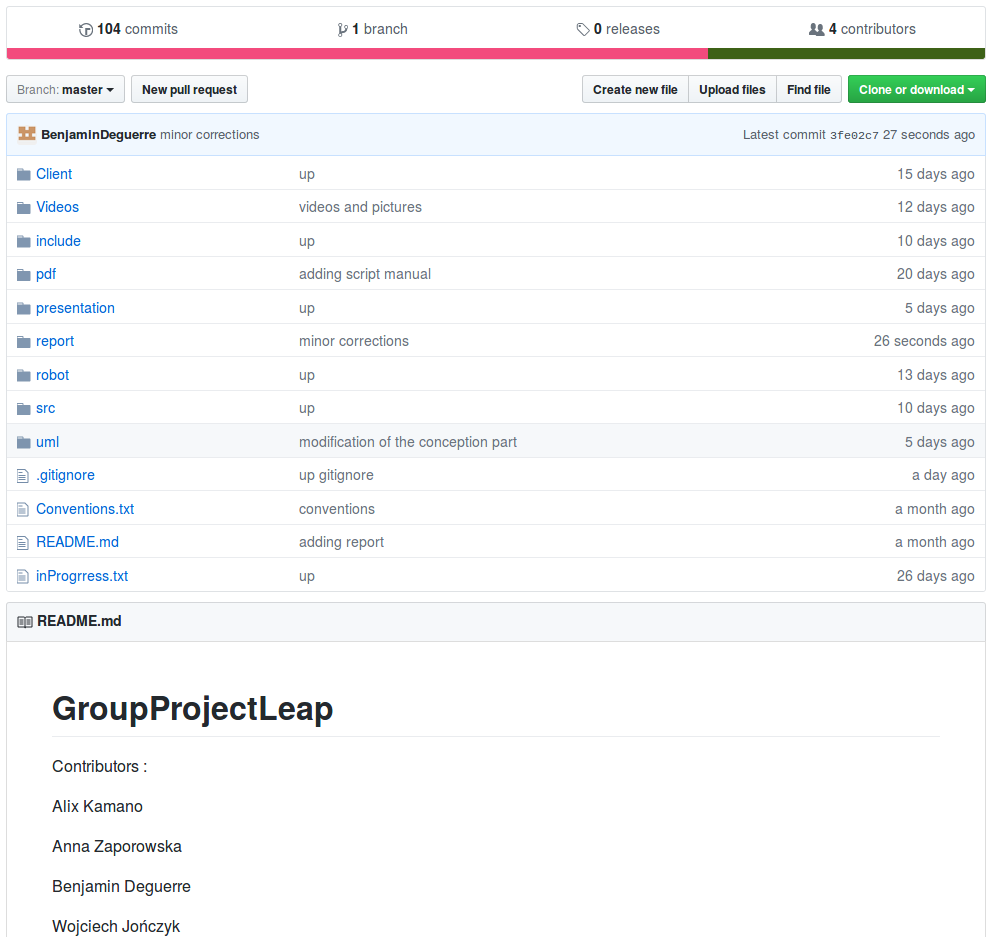
\includegraphics[scale = 0.35]{github}
	\centering
	\caption{GitHub main page of the project}
	\label{fig:github}
\end{figure}

Moreover as it will be shown in the next section, the project was easy to cut down into parts, which makes it perfect for an use coupled with GitHub.

On top of that, GitHub has a system of "branches" and "commit" perfect for a research project. The "branches" let the user try some new algorithm without modifying the main version, and then if the try is succesful, the "branch" can be merge with the main version in order to make it available for each member of the team. As for the commit system, it allows to go back to a previous version of the project in cases of mistakes or even if some previous code is needed due to change within the logic of the program.

\subsection{Group work}

\paragraph{Division of work: \\\\}
We first took some time to think about the structure of the project by using UML diagrams and brainstorming sessions. This let us find the main aim of the project: letter writting and drawing, we wanted the project not to be only a school work, but to have applications in real life. This time spent on the conception made it easier to then divide the work among ourselves. We gave each member of the team a part of the project to develop (functions of the class diagram which will be detailed in the next section).

\paragraph{Conventions: \\\\}

In order to make the work simpler and more efficient, we decided of coding conventions. This may seem irrelevant but it make the work easier by avoiding the problems of translation between the various editors we were using. And because we knew we would not work together it was important not to have this kind of problems each time we try to code something for the project.
